% ==========================================================================
%	RESEARCH PROPOSAL
% ==========================================================================

% - APPROACH ---------------------------------------------------------------
\chapter{Approach}
\label{ch:approach}
% --------------------------------------------------------------------------

This chapter outlines the necessary steps and methodology that is applied in order to achieve the aspired contributions in terms of the desired research goal of this work (\autoref{sec:approach-structure}). This approach definition is not meant to be final and makes no claim to be exhaustive. This is because the practical application of this approach is expected to yield results that either not fit the approach or require extension.

Apart from that, this chapter also identifies underlying assumptions required to perform the work (\autoref{sec:approach-assumptions}) as well as potential risks to the research and their appropriate countermeasures (\autoref{sec:approach-risks})

\section{Research Structure \& Methodology} \label{sec:approach-structure}

In essence, the underlying research methodology will follow an experimental and empirical approach that aims to (i) find limitations and challenges in current frameworks, (ii) develop a unified framework that addresses these issues, and finally (iii) validate its applicability and overall benefit after the fact. The specific measures to be undertaken are outlined in the following.

\subsection{Preparation of Research Environment \& Scope} \label{subs:approach-structure-prepare}

Before pursuing the first contribution of this work, the research environment and scope need to be prepared. Chapters \ref{ch:intro} and \ref{ch:related-work} already established the overall domain under this research will take place, which is \acl{cc}. For that matter, appropriate candidate \ac{cc} offerings and services must be derived in order to have a finite scope of consideration (referred to as $C_{CC_{ofr}}$ and $C_{CC_{svc}}$, respectively). Similarly, this is also the case for the choice of currently used frameworks that solely consider \textit{either} usability \textit{or} security design or evaluation (referred to as $C_{FW_{use}}$ and $C_{FW_{sec}}$, respectively).
Due to limitations in time and scope that come with a Master's thesis, the goal is to have 

\begin{itemize}
	\item three \ac{cc} offerings (denoted as A, B, and C),
	\item five \ac{cc} services (denoted as 1, 2, 3, 4, and 5), as well as
	\item two current usability, and
	\item two current security evaluation or design frameworks.
\end{itemize}

To allow for an independent assessment of the current framework as well as a  controllable validation of the unified framework, the following split is suggested, such that

\begin{itemize}
	\item $A_{CC_{ofr}} \coloneqq \{A,B\} \supset C_{CC_{ofr}}$ defines the assessment set of \ac{cc} offerings,
	\item $A_{CC_{svc}} \coloneqq \{1,2,3\} \supset C_{CC_{svc}}$ defines the assessment set of \ac{cc} services,
	\item $V_{CC_{ofr}} \coloneqq \{B,C\} \supset C_{CC_{ofr}}$ defines the validation set of \ac{cc} offerings,
	\item $V_{CC_{svc}} \coloneqq \{2,3,4,5\} \supset C_{CC_{svc}}$ defines the validation set of \ac{cc} services,
	\item $K_{CC_{ofr}} \coloneqq A_{CC_{ofr}} \cap V_{CC_{ofr}} = \{B\}$ defines the control set of \ac{cc} offerings, and
	\item $K_{CC_{svc}} \coloneqq A_{CC_{svc}} \cap V_{CC_{svc}} = \{2,3\}$ defines the control set of \ac{cc} service. Consequently,
	\item $A_{CC} \coloneqq A_{CC_{ofr}} \times A_{CC_{svc}} = \{A,B\} \times \{1,2,3\} = \{A1,A2,A3,B1,B2,B3\}$ defines the \ac{cc} assessment combination,
	\item $V_{CC} \coloneqq V_{CC_{ofr}} \times V_{CC_{svc}} = \{B,C\} \times \{2,3,4,5\} = \{B2,B3,\dots,C4,C5\}$ defines the \ac{cc} validation combination, and finally
	\item $K_{CC} \coloneqq K_{CC_{ofr}} \times K_{CC_{svc}} = \{B\} \times \{2,3\} = \{B2,B3\}$ defines the \ac{cc} control combination.
\end{itemize}

The total number and setup of the individual candidates is open to discussion and is merely to support the presentation of the upcoming contributions. The concrete candidate choice criteria will be set up during the actual research phase of this work. However, general choice criteria are briefly outlined in the following: 

The choice of offerings will be aided by quantitative indicators (e.g., market share). To allow for comparability, the choice of \ac{cc} services must be done such that each service is similarly implemented and presented across all \ac{cc} offerings. These candidates will then, again, be validated through quantitative indicators (e.g., relevance or popularity).

The choice of current frameworks will solely be done based on its degree of establishment in the corresponding area of application, that is, the most-used design or evaluation frameworks used in either the usability or security domain.

The corresponding \ac{cc} environments will then be set up. These sets of candidates will then serve as the required input for achieving the first contribution C1.

\subsection{C1: Assessment of Current Framework Applicability} \label{subs:approach-structure-assess}
In order to evaluate the applicability of current usability and security design and evaluation frameworks, the candidate sets $C_{FW_{sec}}$ and $C_{FW_{use}}$ will be applied on the \ac{cc} assessment set $A_{CC}$. Specifically, every element of $A_{CC}$ will be individually evaluated by means of all frameworks $C_{FW_{sec}}$ and $C_{FW_{use}}$. This yields the following mapping:

\begin{center}
	$\mathcal{A} \coloneqq A_{CC} \times (C_{FW_{sec}} \cup C_{FW_{use}}) = \{FW_{sec_1}(A1), \dots, FW_{sec_1}(B3), FW_{sec_2}(A1), \dots, FW_{use_1}(A1), \dots, FW_{use_2}(B3)\}$
\end{center}

with $\mathcal{A}$ being the entire set of assessments and its elements being individual assessments mappings of offering service candidates and current frameworks. This yields a total of 24 assessments. Each assessment will be performed manually, noting findings in terms of the usable security applicability for the particular case. It is expected to have the following categories of findings:

\begin{itemize}
	\item pure usability aspects directly related to the application of a usability framework,
	\item pure usability aspects derived from applying a security framework,
	\item pure security aspects directly related to the application of a security framework,
	\item pure security aspects derived from applying a usability framework,
	\item usable security aspects derived from a usability framework, and
	\item usable security aspects derived from a security framework.
\end{itemize}

These categories then yield three applicability degrees:

\begin{enumerate}
	\item aspects that are applicable without change,
	\item aspects that are applicable with change, and
	\item aspects that are not applicable at all.
\end{enumerate}

Furthermore, each assessment is expected to aid the subsequent design process of the unified framework (cf. C2) such that relevant aspects that are missing from the current framework can be derived by justified assumption. After performing each evaluation, the findings and insights can be prioritized in terms of their relevance, how often they appeared, etc.

The results from the control group evaluation will be most thoroughly documented as they will serve as additional input to the validation process of the unified framework (cf. C3).

It is expected that certain cloud services' interfaces do not solely include security aspects, which is why the evaluation will only focus on aspects within the usability that is mostly or entirely security-related.

The ultimate design of this proposed assessment will be revised after deciding on the specific \ac{cc} offerings, services, as well as current frameworks, if necessary. In any case, the output of the total assessment will be subsequently used in the next contribution C2.

\subsection{C2: Design of Unified Qualitative Usable Security Assessment Framework} \label{subs:approach-structure-design}

The findings from C1 are now applied in order to design the unified qualitative usable security assessment framework, as part of the second contribution.

The design will consider the following findings in order:

\begin{enumerate}
	\item High-priority aspects from current frameworks that can be taken over without change.
	\item High-priority aspects from current frameworks that can be taken over with change.
	\item Low-priority aspects from current frameworks that can be taken over without change.
	\item Low-priority aspects from current frameworks that can be taken over with change.
	\item High-priority aspects derived by justified assumption.
	\item Low-priority aspects derived by justified assumption.
\end{enumerate}

After each step, it is validated that the included steps are not redundant to the previously undertaken step. Finally, after performing all steps based on all findings from C1, all aspects are considered in total in terms of consolidation or generalization, if applicable.

Again, the ultimate design of this proposed framework development process will be revised after having the actual assessment of the current frameworks. In any case, this contribution is expected to yield a unified framework that is similar to the mode of application to the previously chosen, current frameworks. This framework is now subject to validation in terms of the third and last contribution C3, outlined in its separate \autoref{ch:evaluation}.

\section{Assumptions \& Limitations} \label{sec:approach-assumptions}
As certain limitations might not be clear until the start of the actual Master's thesis development, this list of assumptions and limitations makes no claim to be exhaustive.

\begin{description}
	\item[Lack of Budget] At the time of creating this research proposal, it is expected that the research to-be-conducted will not receive any financial support which might be beneficial to the evaluation of paid services or offerings. This limits the choice of \ac{cc} offerings and services to free-tier availability. 
	\item[Positioning of \acs{hpe}] This research is conducted in cooperation with the author's employer and requires that their \ac{cc} offering is taken into account. Therefore, one of the supposedly three \ac{cc} offerings must be covered by \textit{\acs{hpe} GreenLake}. 
	\item[Operational Correctness \& Integrity] As this research does not aim at revealing operational issues of the chosen \ac{cc} offerings or services, it is expected that the deployments perform as intended by the provider.
	\item[Agnostic Implementation] In order to allow for general applicability across \ac{cc} offerings, this research does not differentiate between \ac{cc} deployment models for the assessment, development, and validation of the framework(s). Thus, it assumes that the implementation of service configuration interfaces as well as of underlying security features is generally similar.
	\item[Framework Design] The choice of current frameworks is limited to heuristics, guidelines, or principles that do not explicitly define the approach on how they are applied. The goal is to create a unified framework that can be applied on various application approaches and settings (e.g., both moderated \textit{and} unmoderated). This leads to the research not being validated by actual users as the design of application scenarios of the unified framework lies outside the scope of this work.
\end{description}

Overall, further limitations to the scope and complexity of this proposed research are expected as for the given nature of Master's thesis, that is, a limited working time frame of six months, a generally limited amount of content pages (approx. 60-80 pages), and the fact that the work is conducted in a cooperative study manner next to a full-time employment as given by the study program of the HECTOR School.

\section{Risk to the Research \& Mitigation} \label{sec:approach-risks}

As certain risks to this proposed work might not be clear until the start of the actual Master's thesis development, this list of risks and risk mitigations makes no claim to be exhaustive. It does also not contain superior risks outside of the scope of the research and outside the control of the stakeholders (e.g., sickness, emergency situations, etc.). 

\begin{description}
	\item[Misrepresentation of Research Novelty] The analysis of the related work (cf. \autoref{ch:related-work}) has been and will be done to the best of the author's knowledge and belief, especially in terms of describing the present research's limitations. However, it is possible that relevant work is disregarded (e.g., due to unavailability, etc.) that might render this research's contributions less novel than they were expected. In that case, this will be remedied through scope readjustment.
	\item[Misinterpretation of Complexity] During the practical application of the research approach (cf. \autoref{sec:approach-structure}), it is possible that intermediate results yield (i.a.) the unexpected applicability of current frameworks in terms usable security, or, in contrast, their absolute inapplicability, which could distort the expected value of this research. Again, this will be remedied by means of research scope readjustment.
\end{description}


% - ORGANIZATION -----------------------------------------------------------
\chapter{Organization}
\label{ch:organization}
% --------------------------------------------------------------------------

	\section{Research Stakeholders} \label{sec:organization-stakeholders}
	
	The Master's thesis will be conducted by \textbf{Oliver Rudzinski} (oliver.rudzinski@hpe.com).
	\begin{description}
		\item[KIT affiliation] M.Sc. Candidate for Information Systems Engineering and Management at the HECTOR School of Engineering and Management (Technology Business School of the KIT)
		\item[\acsu{hpe} affiliation] Infrastructure Technology Architect for the \textit{Value Solutions} department at the \acl{hpe} Sales Center GmbH in Berlin, Germany. 
	\end{description}
	
	The following stakeholders affiliated with the Karlsruhe Institute of Technology are identified.
		
	\begin{description}
		\item[Reviewer] Prof. Dr. Ralf Reussner (ralf.reussner@kit.edu)
		\item[Second Reviewer] Dr. Robert Heinrich (robert.heinrich@kit.edu)
	\end{description}
	
	Additionally, as the Master's thesis will be conducted in cooperation with the author's employer, the following stakeholder(s) affiliated with \ac{hpe} are identified.
	
	\begin{description}
		\item[Manager] Markus Leitzgen | Inside Sales Manager \textit{Value Solutions} (markus.leitzgen@hpe.com) 
	\end{description}
	
	It shall be noted that additional subject-matter experts, closely related to the \ac{hpe} GreenLake business unit, might be brought in for supporting purposes, or out of interest to their business.	

% --------------------------------------------------------------------------

	\section{Artefacts} \label{sec:organization-deliverables}
	This section outlines the artefacts that are expected to be developed during the process of the Master's thesis. This research proposal document serves as the first artefact. The Master's thesis documentation itself will contain the following artefacts:
	
	\begin{itemize}
		\item description of foundational background to this work (as prepared in \autoref{ch:foundations})
		\item analysis and discussion of related work in the underlying research area (as prepared in \autoref{ch:related-work})
		\item definition of research scope by means of \ac{cc} offerings, services, usability, and security frameworks as well as their classification into assessment, control, and validation sets (as described in \autoref{subs:approach-structure-prepare})
		\item quantified assessment documentation of current frameworks (coinciding with C1, as described in \autoref{subs:approach-structure-design})
		\item unified framework definition (coinciding with C2, as described in \autoref{subs:approach-structure-design})
		\item evaluation of framework and total research approach (coinciding with C3, as described in \autoref{ch:evaluation})
	\end{itemize}
	
	The preliminary versions of these artefacts will be summarized in a presentation that will be held during the thesis' colloquium 4-6 weeks prior to submission. The corresponding presentation slides serve as another artefact to this research.
	
	In case any source code or configuration files are created during the evaluation process of this research, they will be included in adequate manner.
	
	Furthermore, it is expected that the findings of this research will also be presented to an interested audience at \ac{hpe}, which lies outside of the scope of the formal valuation of the thesis.

% --------------------------------------------------------------------------

	\section{Work Schedule} \label{sec:organization-schedule}
	According to the Master's thesis information sheet issued by the HECTOR School, the extent of the Master's thesis for the study program \textit{Information Systems Engineering and Management} is described by 20 ECTS points that correspond to a workload of 600 hours and a development time frame of six months. At the time of this proposal, the official starting date is not yet confirmed. In any case, for the first five months of the thesis development, a rough work capacity of 25 hours per week is expected, which will be increased to 50 hours per week in the last month, excluding the time frames of the remaining HECTOR school modules. This is taken into account for the specific planning of the milestones.
	
	The desired starting date of the thesis development corresponds to the \textbf{1\textsuperscript{st} of October 2022}, which yields the submission date of the \textbf{31\textsuperscript{st} of March 2023}.
	
	It is highly desired to have regular update and mentoring sessions with the reviewers and remaining stakeholders of this research.
	
	\subsection{Work Packages}
	The work packages of this research roughly coincide with the proposed research approach (cf. \autoref{ch:approach}) and evaluation (cf. \autoref{ch:evaluation}).
	
	The preparation work phase (phase 1, cf. \autoref{subs:approach-structure-prepare}) aims at developing criteria for choosing appropriate \ac{cc} offerings and services, followed by deciding on the corresponding elements for this research. Subsequently, this is also done to current security and usability assessment frameworks. Finally, the assessment, validation, and control sets are defined as well as the corresponding \ac{cc} environments prepared. Phase 1 is overlapped by the permanent documentation phase in that the preparatory work is documented as well as the \nameref{ch:foundations} chapter refined.
	
	Phase 1 flows into the assessment phase of current frameworks (phase 2, cf. \autoref{subs:approach-structure-assess}). Before starting with the actual assessment, its proposed approach is refined as well as relevant assessment KPIs defined. Then, the assessments are performed. Findings are derived in parallel to the assessments, and finalized by means of a total assessment insight priorization. As before, the documentation phase overlaps in that the entire process is documented. \nameref{ch:related-work} refinement is also done in that phase.
	
	Phase 2 then flows into the design phase of the unified framework (phase 3, cf. \autoref{subs:approach-structure-design}) with the evaluation of the total findings from phase 2. With that, the framework design approach can be refined, if necessary, that is subsequently used for the actual development of the unified framework. Upon finalizing the framework, it is thoroughly examined in terms of redundancy, possibility of abstraction, etc. Again, the documentation phase runs in parallel by documenting the design approach refinement as well as the actual process of framework development. Further potential \nameref{ch:foundations} and \nameref{ch:related-work} refinement is also done in that phase.
	
	Phase 3 flows into the last practical work phase of evaluating the new framework as well as the entire approach (phase 4, cf. \autoref{ch:evaluation}). This, again, starts with a potential refinement of the evaluation strategy, followed by the comparative evaluation by means of the control set as well as the validation of general applicability via the validation set. Again, the evaluation is documented in parallel.
	
	Phase 4 finally flows into the now solely present documentation phase. Here, the preliminary documentation is refined in terms of structure, wording, conciseness, etc., resulting in a first completed draft that will be presented during this thesis' colloquium. The feedback received during the presentation will finally be applied to the work, before final proof reading and formatting takes place. Finally, the thesis is completed, printed, and submitted for grading.
	
	\subsection{Milestones}
	The milestones of this work generally coincide with the end of each major work phase and work artefacts, which are defined as follows:
	
	\begin{description}
		\item[Phase 1] completed choice of \ac{cc} offerings, services, and current framework candidates and corresponding mappings into assessment, validation, and control sets
		\item[Phase 2] derived findings and insights on current framework assessment in terms of usable security
		\item[Phase 3] final definition of unified qualitative usable security assessment framework
		\item[Phase 4] final findings of unified framework and total research evaluation, as well as final derivation of limitations and research outlook 
		\item[Documentation Phase] divided into two milestones: (i) perform colloquium presentation, as well as (ii) submission of Master's thesis
	\end{description}
	
	In \autoref{subs:organization-work-gantt} on the next page, a  GANTT chart represents the described work phases and corresponding milestones of the Master's thesis development. 	\\\ This concludes the research proposal.
	
	\subsection{GANTT Chart} \label{subs:organization-work-gantt}
	\begin{center}
		\vfill
		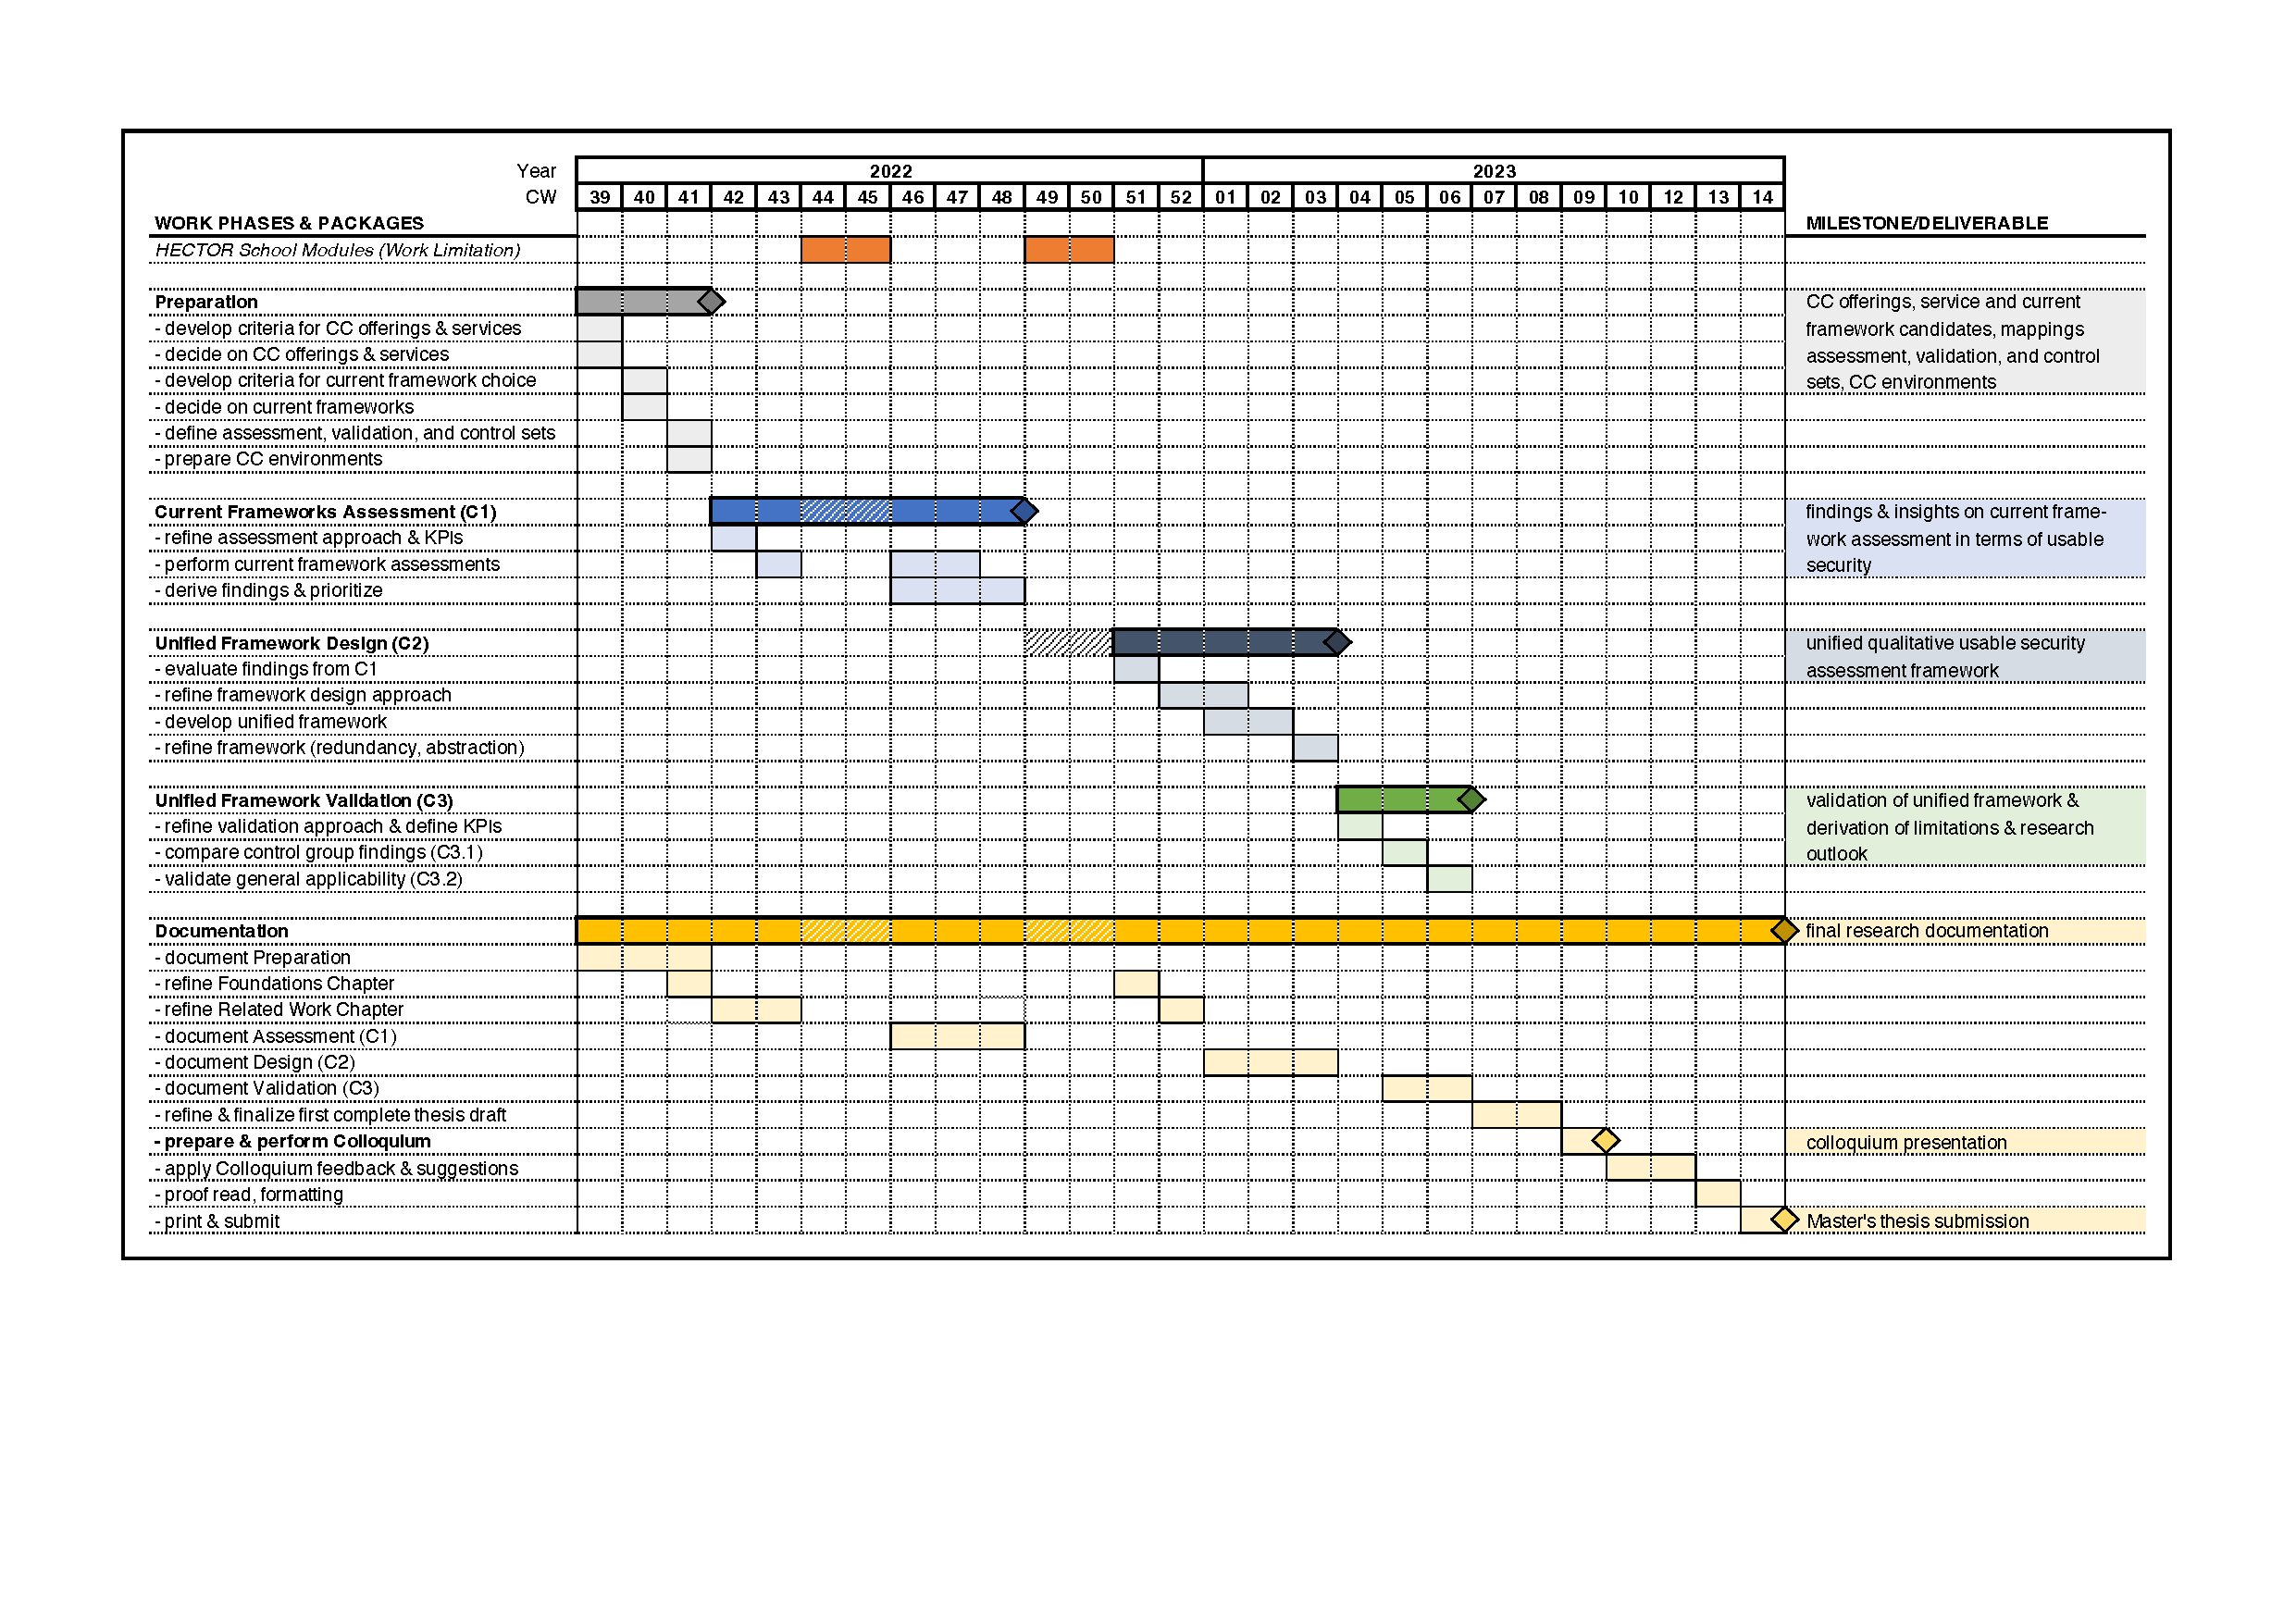
\includegraphics[angle=90,scale=0.58]{content/2-research-proposal/img/gantt.pdf}
		\vfill
	\end{center}
	\newpage